\documentclass[twocolumn]{article}
\setlength{\columnsep}{20pt}
%\usepackage{url}
%\usepackage{algorithmic}
\usepackage[a4paper]{geometry}
\usepackage{datetime}
\usepackage[font=small,labelfont=it]{caption}
\usepackage{graphicx}
% Use Times NR as font
\usepackage{lmodern}
\usepackage[T1]{fontenc}

\usepackage{float}

% Better tables
\usepackage{tabularx}
% to make beautiful tables
\usepackage{booktabs}

\usepackage{microtype}
\usepackage{amsmath}
\usepackage{subfigure}

% Letterspacing macros
\newcommand{\spacecaps}[1]{\textls[200]{\MakeUppercase{#1}}}
\newcommand{\spacesc}[1]{\textls[50]{\textsc{\MakeLowercase{#1}}}}

\title{\huge{\textbf{Study doc: tile size experiment}}\\ \normalsize \Large{how does the size of the audio segments affect the embedding space}}

\author{Fabian Gröger\\fabian.groeger@stud.hslu.ch}
\date{\today}

\begin{document}
\maketitle

\begin{abstract}
The experiment aims to show the effect of the size of the audio segments which will be used as the size of the triplets.
\end{abstract}

\section{Introduction}
The size of each triplet, which will be fed to the network, is an essential hyperparameter which needs to be carefully chosen. Because it specifies how much information each segment contains and is therefore fed to the network. If the segments are chosen too small, it does not contain enough information to distinguish between categories. If the size is too big, the segment contains too much information, and therefore, the model needs to work with a lot more data and gets a lot heavier. This experiment is conducted to search an optimal segment size for the triplets.

\section{Hyperparameters}
The hyperparameters used for this experiment are shown in table \ref{tab:Hyperparameters}. The experiment will be conducted using a state of the art ResNet18 architecture on the DCASE dataset. The hyperparameters in section \textit{Feature representation} as well as the sample rate are the default ones proposed by the organisers of the DCASE challenge within the baseline project. The sample tile size will be evaluated for three different values \texttt{[1, 2, 4]} in seconds.

\begin{table}[H]
    \centering
    \caption{Hyperparameters used for the experiment}
	\label{tab:Hyperparameters}
    \begin{tabular}{l|l}
        \toprule
        \textbf{Hyperparameter} & \textbf{value} \\ 
        \midrule[1pt]
        Dataset & DCASE \\
        \hline
        Model & ResNet18 \\ 
        \hline
        Epochs & 20 \\ 
        \hline
        Batch size & [32, 256] \\ 
        \hline
        Optimizer & Adam \\ 
        \hline
        Learning rate & 1e-4 \\
        \hline
        Margin & 1.0 \\
        \hline
        L2 regularisation amount & 0.0 \\
        \hline
        Embedding dimension & 512 \\
        \hline
        Prefetch batches & Autotune (-1) \\ 
        \hline
        Random selection buffer & 64 \\ 
        \hline
        Shuffle dataset & True \\
        \hline
        Random seed & 1234 \\
        \midrule[1pt]
        \multicolumn{2}{l}{\textit{Multi threading}} \\
        \midrule[1pt]
        Number of generators & 16 \\ 
        \hline
        Number of parallel calls & 16 \\
        \midrule[1pt]
        \multicolumn{2}{l}{\textit{Audio sample}} \\
        \midrule[1pt]
        Sample rate & 16000 \\ 
        \hline
        Sample size & 10 \\
        \hline
        Sample tile size & [1, 2, 5] \\
        \hline
        Sample tile range & [4, 5] \\
        \hline
        Convert to mono & True \\
        \midrule[1pt]
        \multicolumn{2}{l}{\textit{Feature representation}} \\
        \midrule[1pt]
        Feature extractor & LogMelExtractor \\ 
        \hline
        Frame length & 480 \\
        \hline
        Frame step & 160 \\
        \hline
        FFT size & 1024 \\
        \hline
        Number of Mel bins & 128 \\
        \hline
        Number of MFCC bins & 13 \\
        \bottomrule
    \end{tabular}
\end{table}

\begin{figure}[t]
\centering
    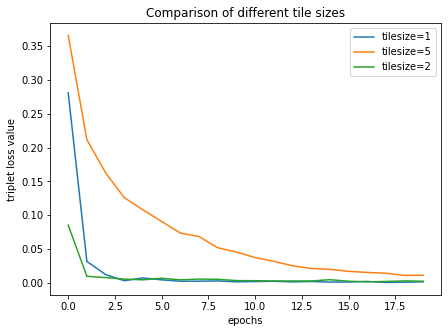
\includegraphics[width=\linewidth]{assets/tile_sizes_plot.png}
    \caption{Plot of the triplet loss of the different tile sizes}
    \label{fig:tile-size-plot}
\end{figure}

\section{Results}
Three models with the same hyperparameters, shown in table \ref{tab:Hyperparameters}, were trained for 20 epochs. The value of the triplet loss is the primary evaluation criteria which will be used to compare the different triplet sizes since it has the most effect on this value because it should show how much of an audio sample is needed to distinguish between different classes. Figure \ref{fig:tile-size-plot} shows all the trained models in a single plot to visualise the impact of changing the sample size. Nevertheless, it is quite hard to interpret the different graphs since all of them are near zero.

The figure \ref{fig:tile-size-plot} shows that the tile size 5s has the highest loss value while the tile sizes 1s and 2s have relatively similar values. However, this does not mean that the tile size of 5s is the worst out of the three, it instead means that the model finds it harder to distinguish audio files when a larger sample is available, which is pretty evident since longer samples also contain more information.

The figure \ref{fig:tile-size-plot} also shows that the tile sizes of 1s and 2s have a very steep graph at the beginning and then hardly change their value. This indicates that it is relatively simple to achieve a good loss value with small audio samples, which means that the model can easily distinguish between small samples.

Both of these interpretations of the plot is pretty straight forward, but when the resulting embedding space is further examined using the Embedding Projector from the tensorboard, it can be seen that the tile size of 5s (\ref{fig:embedding-5s}) results in much clearer clusters than the tile size of 1s (\ref{fig:embedding-1s}). 

\begin{figure}[t]
\centering
    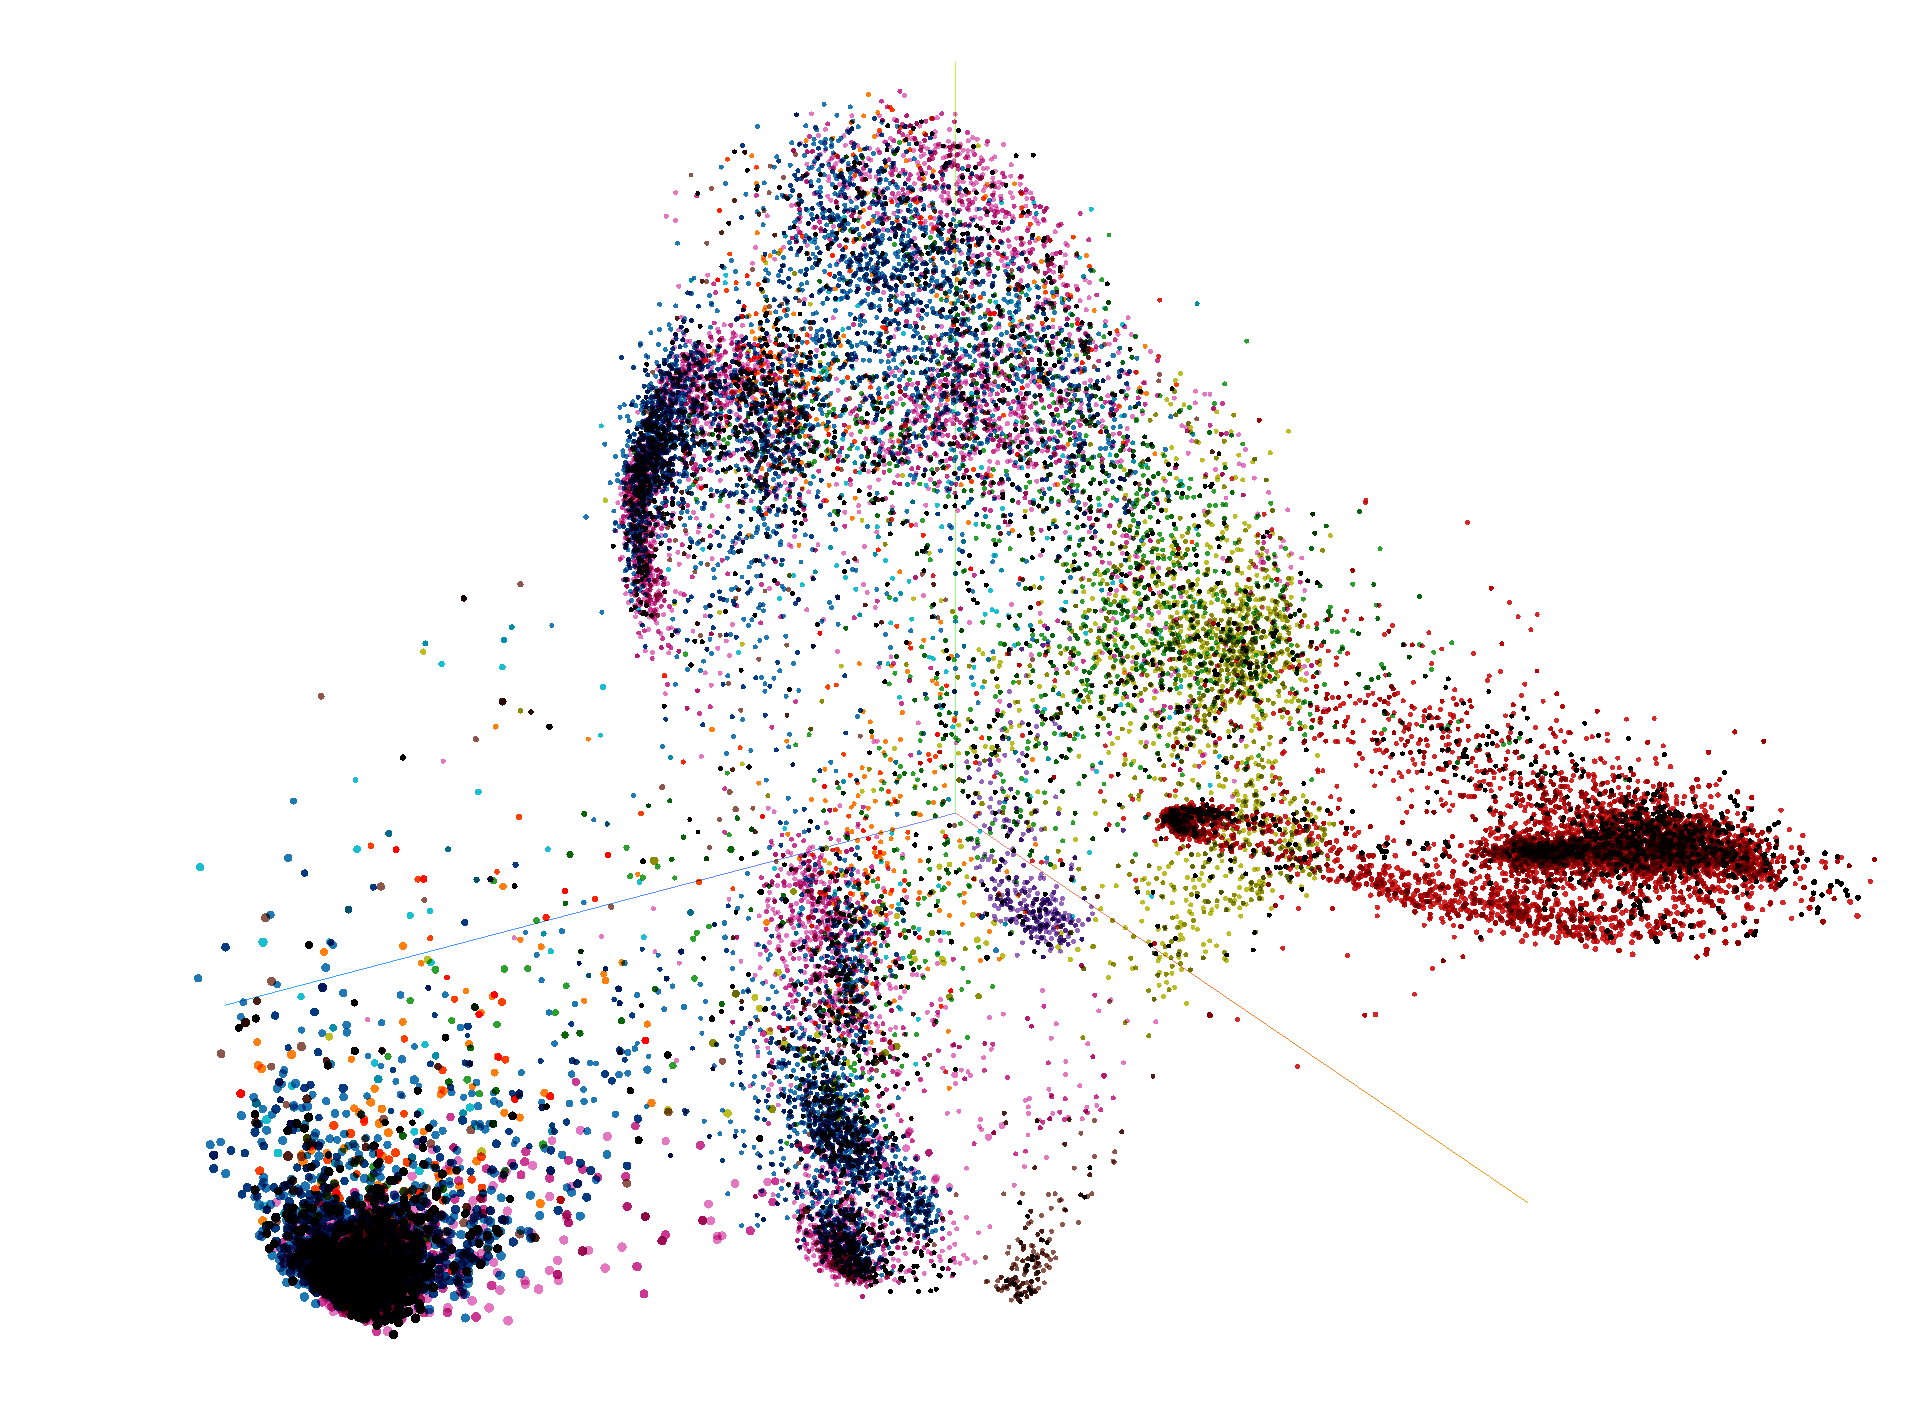
\includegraphics[width=\linewidth]{assets/embedding_space_5s.png}
    \caption{Visualisation of the embedding space from the tile size 5s}
    \label{fig:embedding-5s}
\end{figure}

\begin{figure}[t]
\centering
    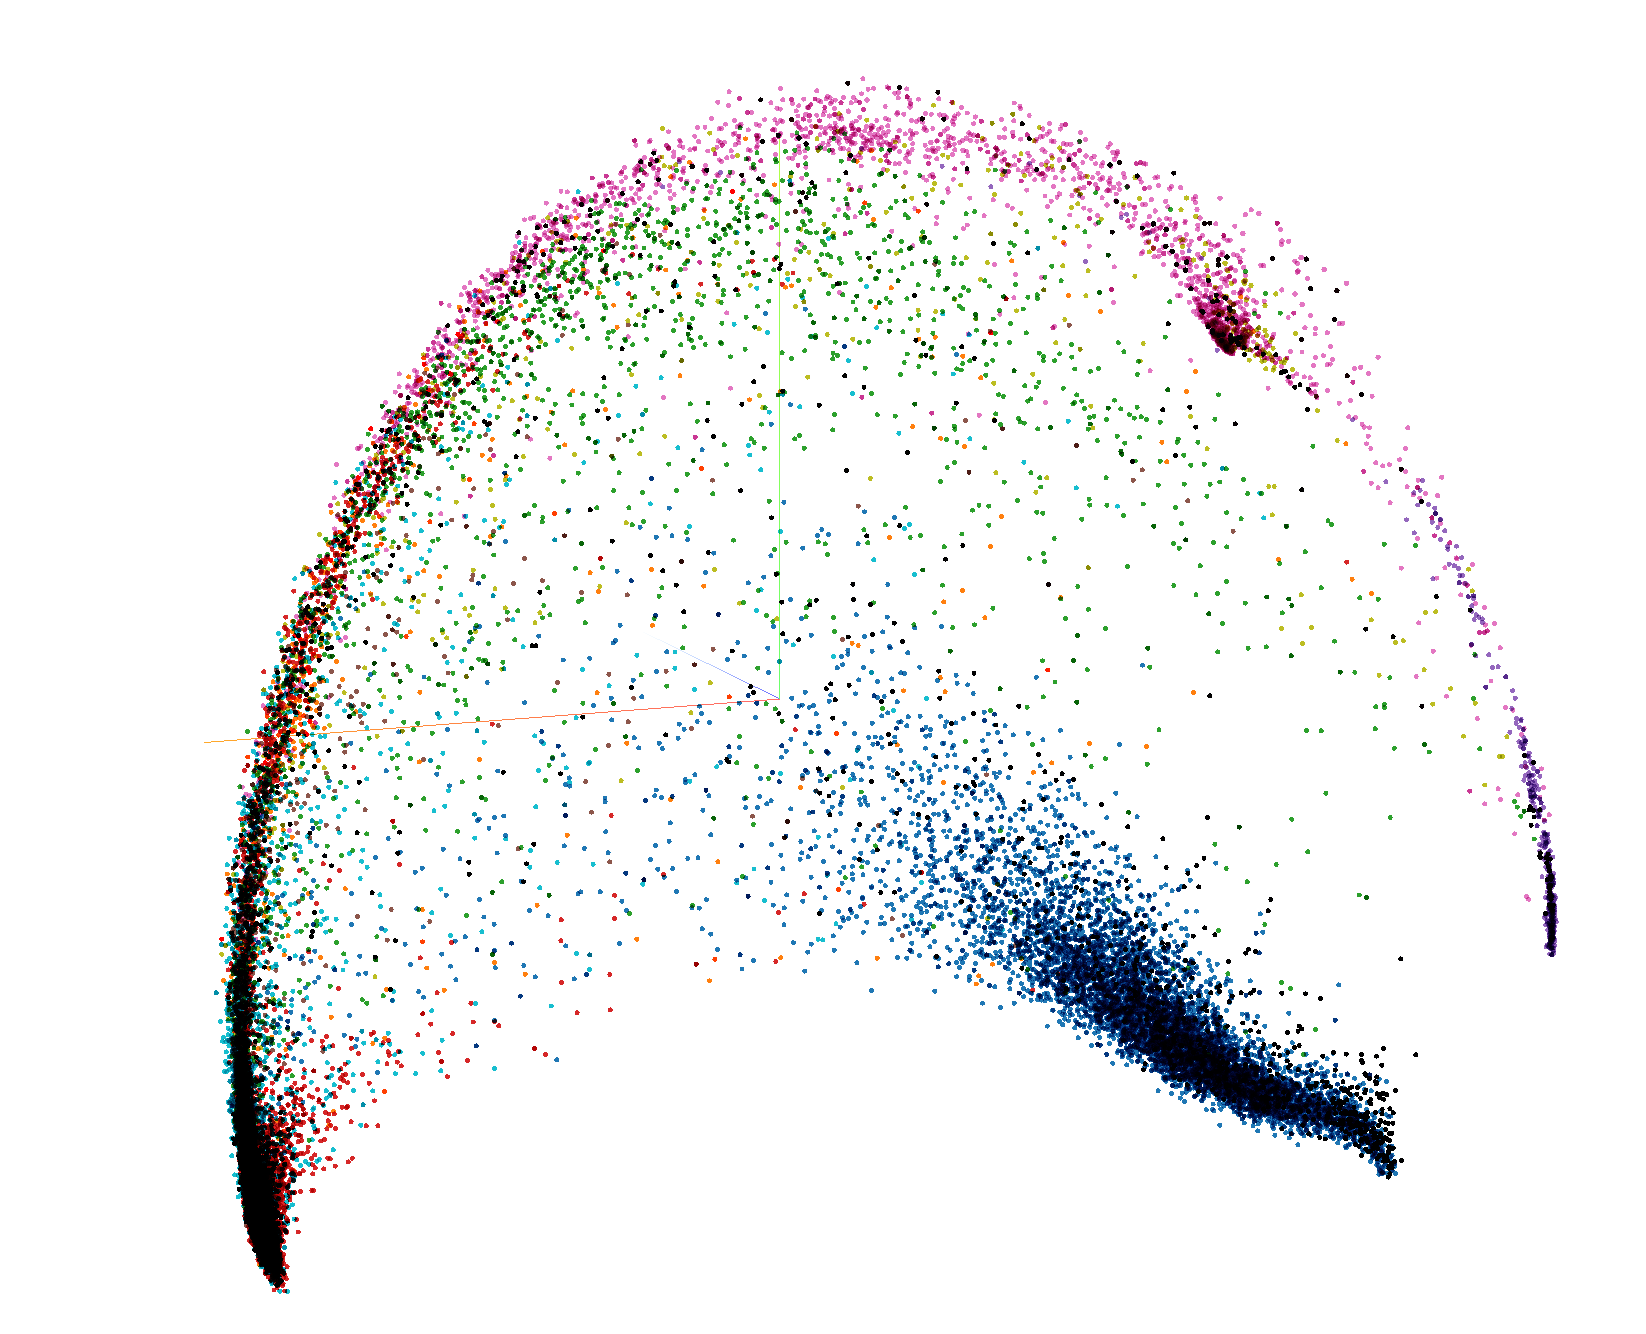
\includegraphics[width=\linewidth]{assets/embedding_space_1s.png}
    \caption{Visualisation of the embedding space from the tile size 1s}
    \label{fig:embedding-1s}
\end{figure}

\section{Conclusion}
If the optimal parameter for the sample tile is only chosen from the loss value and therefore, from the plot \ref{fig:tile-size-plot}, it would be quite hard. However, since the visualisation of the embedding space shows a clear benefit in using a larger sample, the \textbf{sample tile size of 5s} is chosen to be the optimal one for the DCASE dataset. This can be explained because smaller samples much often contain sounds which do not indicate a specific sound in that class, say for example there is a two-second silence in a sound file of the class eating, it would be projected in the nearby region of silence in a sound of a different class, which is useful for other applications but since the goal is to achieve a best possible embedding space, this is not a satisfying result. Therefore, the larger sound segments are more robust to such problems, since they hold much more information about the resulting class. 

If the thesis focused on supervised triplet loss, it would make sense to cut the audio files in much smaller segments than in the unsupervised setting, since in supervised learning the triplet selection makes sure that the clustering focuses on the classes and not some other arbitrary criteria, which happens in unsupervised learning. In the unsupervised triplet loss, it is challenging to examine what exactly is being clustered, because there can be an underlying structure which can not be seen for us humans.

\section{Next steps}
The experiment has found an optimal parameter for the dataset and will be used from now on for the next experiments.

\end{document}